\section{Introduction}

Preventable Medical Errors (\PMEs{}) characterized by
incorrect intended treatment, or incorrect executions of intended
treatment present a significant challenge in Healthcare
\cite{RodziewiczStatsPearls18}. According to a seminal report on the subject
\cite{DonaldsonBook00}, in 1997,
between 44,000 and 98,000 deaths were estimated to have been caused by \PMEs{} in
the United States alone. A more recent study analyzed data from the eight-year
period between 2000 and 2008, and estimated that in 2013, the number of deaths
caused by \PMEs{} was more than 250,000, making \PMEs{} the third-leading
cause of death in the United States \cite{MakaryBMJ16}.
The adverse effects of \PMEs{} extend beyond patient outcomes.
One study estimated the financial burden of \PMEs{} to the United States to be
19.5 billion dollars in 2008 \cite{AndelJHCF12}. According to the authors of
\cite{RodziewiczStatsPearls18}, \PMEs{} caused psychological effects such
as anger and guilt in healthcare providers (\HCPs{}), adversely impacting their mental
health.

One strategy to mitigate \PMEs{} is to utilize evidence-based statements
published by hospital and medical associations that codify recommended
interventions for various clinical scenarios called Best Practice Guidelines (\BPGs{})
\cite{field1990clinical}. High quality guidelines are routinely updated to account for
 results from clinical trials and advances in medicine, and make the latest
 diagnosis and treatment information accessible to providers \cite{SteinbergNAP11}.

While \BPGs{} have the potential to reduce medical errors, their effectiveness hinges
on the adherence of healthcare providers to them.
For example, consider Advanced Cardiac Life Support (\ACLS{}): a \BPG{} published
by the American Heart Association (AHA) for management
of a life threatening condition called in-hospital cardiac arrest (IHCA) \cite{AHAGuidelineAdult, AHAGuidelinePed}. Studies suggest that management
of IHCA in 30\% of adult, and 17\% of pediatric cases deviates from the
AHA-prescribed \BPG, resulting in worse patient outcomes \cite{Ornato2012DeviationAdult,Wolfe2020DeviationPediatric,
Crowley2020DeviationAdult,Honarmand2018Adherence,Mcevoy2014Adherence}.


While \BPG{}-adherence is difficult to achieve in
practice \cite{RandJAMA99,DavisCMAJ97},
integrating \BPGs{} with existing patient care-flow,
and making them readily-accessible when required can improve adherence \cite{WoolfBMJ99}.
To this end, hospitals commission computerized Decision Support Systems (\CDSSs{})
that codify \BPGs{} and support \HCPs{} with situation-specific advice.
Such systems have been shown to improve \BPG{}-adherence \cite{GargJAMA06,KawamotoBMJ05}, and evidence from multi-center clinical trials
suggests that they reduce \PMEs{} \cite{BenettJAMIA16,SahotaJIS11}.
Thus, guideline-based \CDSSs{} are now considered imperative to the
future of medical decision making in general \cite{JamesNEJM01}.

We briefly provide an overview of existing research on \CDSSs{} to explain why
it doesn't addressed problems we intend to address in this proposal.
There exists a large body of research on \CDSSs{}. In
\cite{PelegJBI13}, the author provides a methodological review of
existing work on Computer Interpretable Guidelines (\CIGs{}): executable
formalizations of \BPGs{} used to construct \CDSSs{}.
Existing work is classified into one of eight themes spanning
the entire development cycle of a \CIG{}. The themes and relations between them
are shown in \figurename{} \ref{fig:cpg-research-topics}.

\begin{wrapfigure}{l}{0.5\textwidth}
  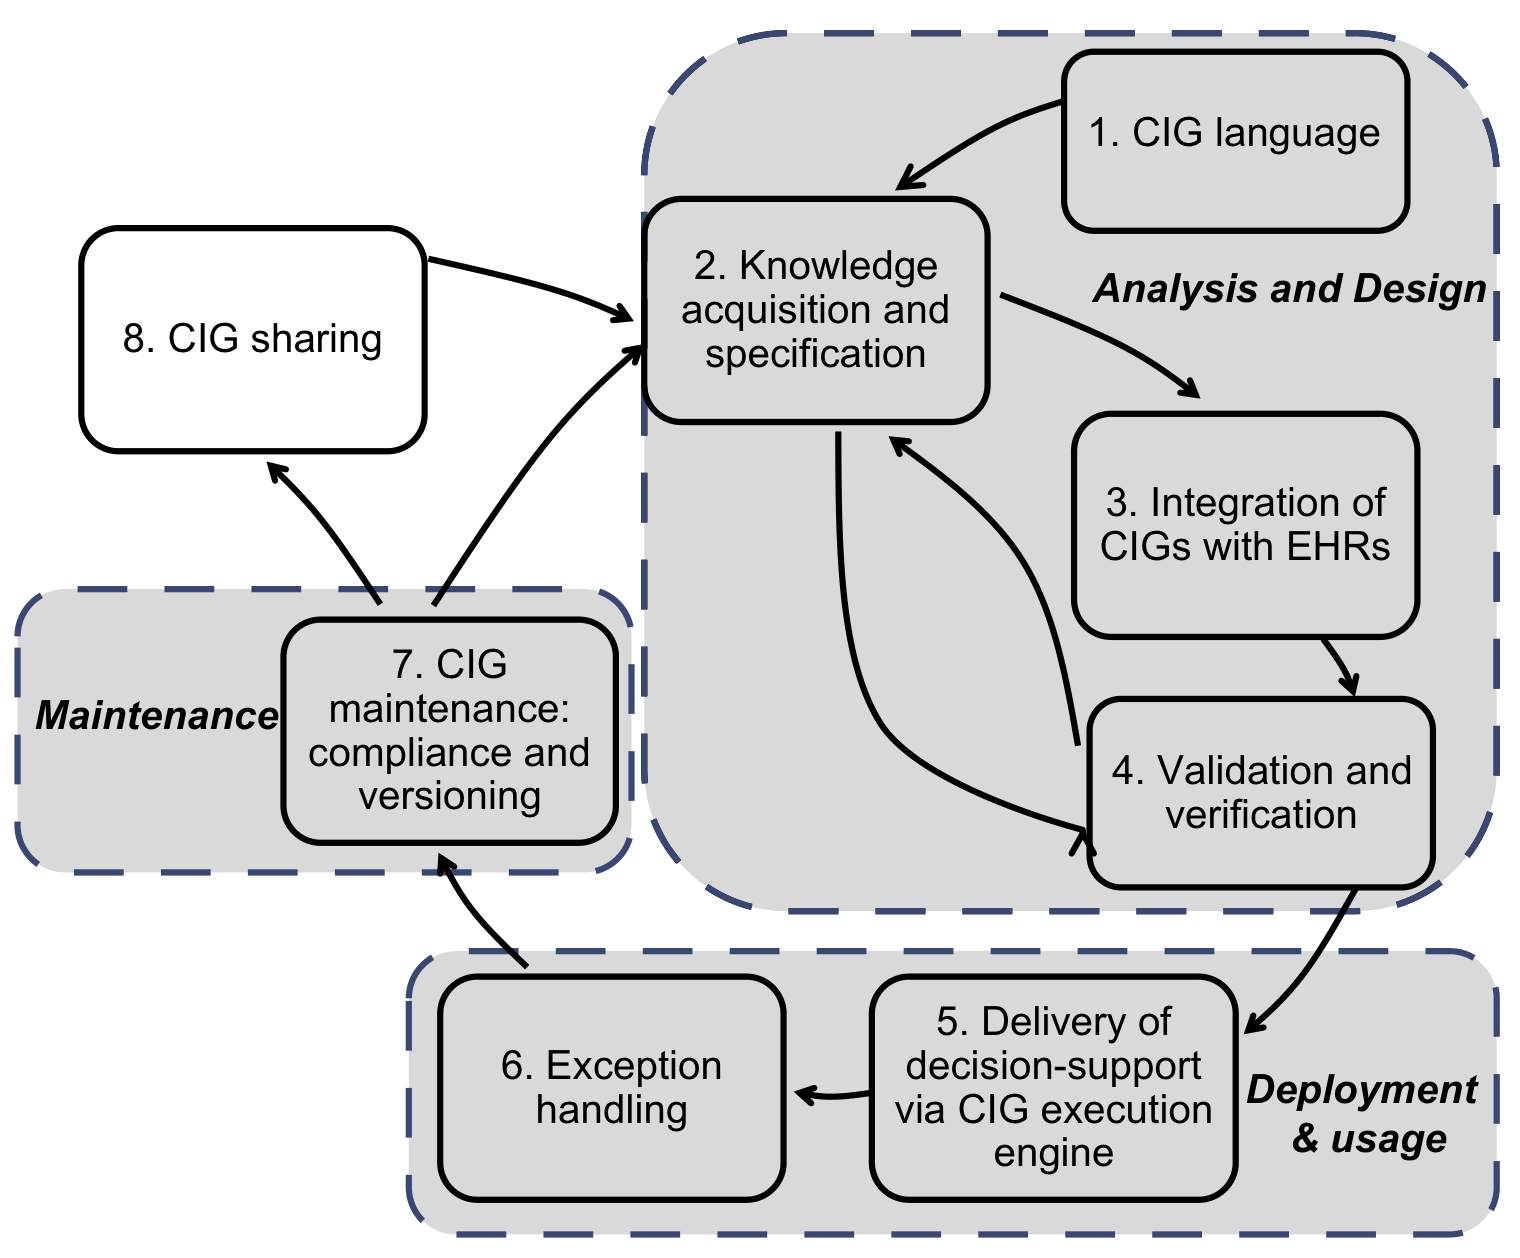
\includegraphics[width=\linewidth]{cpg-topics}
  \caption{\CDSSs{} Research Themes}\label{fig:cpg-research-topics}
\end{wrapfigure}

According to the author in \cite{PelegJBI13}, \CIGs{} are usually based on previously published non-executable
\BPGs{}. To develop a \CIG{}, a language is identified in (1). Teams of
software developers and clinicians then collaborate to express medical knowledge
in the \BPG{} in the identified language. In (3), the \CIG{}
is integrated with components such as a Graphical User
Interface (\GUI{}), Electronic Health Records (\EHRs{}) and external devices
(such as monitors for patient parameters) to obtain a \CDSS. Before adoption
in the real-world, it is imperative to ensure that the \CIG{} \emph{mirrors}
the underlying \BPG{}. This validation occurs by \emph{testing} the \CDSS{}
using execution capabilities of the modeling language from (1) in (5).
Additionally, formal verification may be used to establish other desired
properties hold. Inconsistencies identified in (5) are fixed through developer-clinician
collobaration in (2),  re-validation and
verification. While the aforementioned development cycle has resulted in several
effective \CDSSs{}, it has some limitations:

\paragraph{Gap between specification and implementation:}

To develop the \CIG{}, software developers rely on clinicians to interpret the
non-executable \BPG{} and communicate
the intended semantics to them. Thus, the non-executable \BPG{} serves as a functional specification for
the \CIG{}, i.e. the implementation. In such safety-critical systems, it is
imperative that the implementation, i.e. the \CIG{}, conforms to its
specification, i.e., the \BPG{}. To address this, the \CIG{} is tested by
putting the \CDSS{} through clinical simulations. But, while testing reduces
the risk of non-conformance, it does not completely eliminate it.

\paragraph{Safe Modularity:}

While developing \CDSSs{} is both complex and cost-intensive,
the development effort can be reduced by sharing \CDSSs{} across hospitals \cite{PelegAMIA00}.
But, even for the same \BPG{}, hospitals develop their own \CDSSs{} to address
their needs, resulting in duplicated work.
For instance, for the \ACLS{} \BPG{}, multiple \CDSSs{} have been developed by different
different hospitals in a span of just six years years \cite{FullCodePro,PediAppRREST2020,
PediAppRREST2021,GuidingPad2017,GuidingPad2019, GuidingPad2020,DST2014,DST2019,ROSCo2021,TeamScreen2019,Wu2017}.
\CDSSs{} based on the same \BPG{} typically have the same \CIG{}, but may differ
in their Graphical User Interfaces (\GUIs), or integration with external
devices, to address hospital-specific needs.
To enable safe sharing of knowledge, we need a mechanism that:
\begin{enumerate*}[label=(\alph*)]
  \item allows a stable, formally-verfied \CIG{} that is \emph{decoupled} from other
    components, and,
  \item supports hospital-specific customizations without compromising system
    \emph{safety}.
\end{enumerate*}

\paragraph{Holistic System Safety:}

Actions performed by a \CDSS{} can either be \emph{programming-oriented}
or \emph{clinically-oriented} \cite{BoxwalaJBI04}. \emph{programming-oriented}
actions are peformed by executing the \CIG{} itself. For example,
using patient parameters, or health records to make a reccomendation or diagnosis,
or to raise a warning. \emph{clinically-oriented} actions on the other hand
are ones that involve a clinician. For example, in the case of \ACLS{},
the \CDSS{} recommends that Cardiopulmonary Resuscitation (\CPR{}) be performed
for a certain length of time. Such actions can only be performed by clinicians,
an the \CDSS{} assumes that the recommended action was indeed performed before
moving resuming guidance.

For holistic system safety, both categories of actions must be completed
successfully. While traditional formal reasoning techniques can be employed
to establish correctness of \emph{programming-oriented} actions, the same
cannot be used to reason about \emph{clinically-oriented} ones.
Thus, a mechanism that allows some guarantees about clinically-oriented is
desirable.


\paragraph{Formal Semantics:}

Since \CIGs{} are safety-critical, it is vital that the
language in which they're developed has complete formal semantics that
can be used to derive tools such as semantically-correct interpreters,
deductive program verifiers, and model-checkers.

%Thus, guideline-based \CDSSs{} are now considered imperative to the
%future of medical decision making in general \cite{JamesNEJM01}.
%A guidelines-based \CDSS{} typically consists of:
%\begin{enumerate*}[label=(\roman*)]
%  \item a translation of the guideline to an executable medium, called the
%  \BPGLogic{},
%  \item an interface for user-interaction, and,
%  \item additional infrastructure that integrates with external data sources
%  such as sensors, health records \cite{SuttonNature20}.
%\end{enumerate*}
%Typically, to develop a \CDSS{}, domain experts in medicine
%collaborate with computer scientists to develop requirements documentation
%that presents the \BPGs{}'s
%semantics in a manner amenable to software development \cite{PelegJBI13}.
%This documentation is then utilized to develop the \BPGLogic{}, which is subsequently integrated with data sources (such as patient-parameter sensors and health records),
%and a User Interface (UI) to obtain a complete system. Thus, the \BPG{}
%serves as a functional specification for the \CDSS{}'s \BPGLogic{}.
%But, the aforementioned process has several limitations.
%First, the implementation, i.e., the \BPGLogic{} may not concur with its specification,
%i.e., the text-based \BPG{}. \BPGs{} are specified as long, complex textual documents,
%where the exact meaning of terms may not be explicitly stated, and recommendations may be ambiguous \cite{ClerqAIM03}.
%Capturing and communicating these complexities via requirements documentation
%is challenging, and incorrect or incomplete documentation has resulted in failed
%implementations \cite{KubbenBook19}. Second, as \BPGs{} evolve to reflect
%new evidence or local adaptions, corresponding updates must be made to the
%\CDSS{} as well. However, due to the gap between the \BPG{} and the \BPGLogic{},
%effort must be expended into bringing the \BPGLogic{} to reflect said updates.

\subsection{Limitations of Existing Approaches}

While existing approaches have been imperative to increasing \CGS{} adoption, to the
best of our knowledge, none of them address all of the aforementioned
limitations. We briefly describe notable approaches, their successes, and their limitations.

The Arden Syntax \cite{HripcsakCBM94} a widely used medium for
expressing \CIGs{}.  Guidelines as described using Medical
Logic Modules that contains information related to guideline's purpose
, maintainance, and medical knowledge. The modules are modular to allow
re-use and sharing across hospitals. But, Arden Syntax
is focused on describing simple, modular, and independent
guidelines (such as reminders), and not on guidelines with complex logic (such
as treatment protocols) \cite{PelegJBI01}.
Arden Syntax's limitation in modeling complexity is addressed by
GLIF \cite{BoxwalaJBI04}: a language that uses flowcharts to expressed
guidelines. A multi-level approach is
employed to manage complexity: at the top is the conceptual level, where
only high-level details relevant for human-comprehension are present. In the
middle is a computable-level, where details of guideline execution flow
and patient data elements are specified. At the bottom is the implementable
level, where institution-specific details and mappings into patient data are
specified. Both Arden Syntax and GLIF  eliminate
the gap between the \BPG{}, i.e. the specification, and the \CIG{}, i.e. implementation as
they're meant to be either directly used by clinicians (or in collaboration with
computer scientists) to express \BPGs{} in an executable medium. \CIGs{}
expressed in them are meant to be shared across hospitals, and are thus modular.
However, neither formalism has complete formal semantics, or comprehensiev support for
rigorous formal analysis.

The need for formal analysis is identified by Asbru: a formalism with formally
defined syntax and semantics \cite{ShaharAMIA96}. In Asbru, a guideline is modeled as a plan
that contains:
\begin{enumerate*}[label=(\roman*)]
  \item intentions that define aims,
  \item conditions that specify when the plan is applicable,
  \item effects that define expected behavior during execution, and,
  \item a body containing other subplans.
\end{enumerate*}
Apart from an execution engine, the Asbru ecosystem also contains
other tools, such as a model checker for verification \cite{BaumlerSPIN06}.
However, the formal semantics of Asbru have been only partially defined, and
is insufficient to implement tools for the language \cite{SuttonAMIA03}.
The importance of a complete formal-semantics is identified and addressed
by PROforma \cite{SuttonAMIA03}, another formalism that uses plans to
model guidelines. A PROforma plan is made of a sequence of tasks.
The plan defines constraints on their enactment, and circumstances
for termination (for example, exceptions) \cite{SuttonAMIA03}. But, despite
having complete formal semantics, it does not have a comprehensive suite of
formal analysis tools such as model checkers, deductive verifiers.


The SAGE guideline model \cite{TuSAGE04} uses the Prot\'eg\'e knowledge
representation framework \cite{NoyAMIA03} to model guidelines,
and improves on aforementioned approaches by
enabling seamless integration into hospitals' existing Clinical Information Systems
(\CISs). But, it lacks complete formal semantics, and analysis tools
such as deductive verifiers and model checkers.
The GLARE formalism \cite{TerenzianiBook04} uses an actions based approach
to represent guidelines, and addresses clnician-comprehensibility and
modularity. For formal analysis, GLARE guidelines can be translated to
Promela: the SPIN model checker's specification language \cite{GiordanoAMIA06}.
The approach partly addresses holistic safety as
external agents (such as clinicians) can be modelled and analyzed.
But, the scenario where the external agent's behavior
deviates from the model during system execution isn't addressed.
Non medical-domain specific languages can also be used to reason about
medical systems. For example, in \cite{ArcainiMEMCODE15}, Abstract State
Machines (\ASMs) are used to validate and verify a system for measuring
patients' stereoacuity in the diagnosis of amyblyopia. But such a
formalism, while suitable for formal verification, may
not be easily comprehensible to clinicians for validation.

In \tablename{} \ref{table:existing-approaches}, we provide an overview of
the strengths and limitations of existing approaches. Note that we use
\greencheck{}, \cancelcheck{}, and \redcross{} to depict that an approach
fully-addresses, partly-addresses, or doesn't address a limitation respectively.
To the best of our knowledge,
none of the aforementioned approaches have:
\begin{itemize}[leftmargin=*]
  \setlength\itemsep{0em}
  \item An interpreter or execution engine with \emph{\underline{correctness guarantees}}.
  \item A Rich Suite of \emph{\underline{formal analysis tools}} such as a deductive program
    verifier, model checker, and symbolic execution engine that can be used to
    reason about the guidelines. Since a \CIG{} can comprise multiple
    processes that are \emph{parallel}, \emph{sequential}, or a mix of both,
    reasoning about them can be challenging. But, existing work in modeling
    and reasoning about distributed systems can provide solutions.
  \item Ability to reason about agents that perform \emph{\underline{external
    agents}}. These include clinicians responsible for \emph{clinically-defined}
    actions, or \emph{monitors} for \emph{patient parameters}. While it may seem
    impossible to reason about systems that depend heavily on actions of
    external agents, solutions to similar problems in other domains, such as
    the Simplex Architecture \cite{BakRTAS09} in Real-Time Systems (\RTSs), can be looked at for directions.
\end{itemize}

\begin{center}
\renewcommand{\arraystretch}{0.5}
%\setlength\extrarowheight{-9pt}
  \begin{table}
  \begin{tabularx}{\textwidth}{
      >{\centering\arraybackslash}X
    || >{\centering\arraybackslash}X
    | >{\centering\arraybackslash}X
    | >{\centering\arraybackslash}X
    | >{\centering\arraybackslash}X
  }
                 & Implementation-Specification Gap & Complete Formal Semantics & Formal Analysis Tools & Holistic Safety  \\
    Arden Syntax & $\greencheck$                               & $\redcross$               & $\redcross$           & $\redcross$ \\
    GLIF         & $\greencheck$                               & $\redcross$               & $\redcross$           & $\redcross$ \\
    Asbru        & $\greencheck$                               & $\cancelcheck$            & $\greencheck$         & $\redcross$ \\
    PROForma     & $\greencheck$                               & $\greencheck$             & $\redcross$           & $\redcross$ \\
    GLARE        & $\greencheck$                               & $\cancelcheck$            & $\cancelcheck$        & $\cancelcheck$ \\
    Promela/SPIN & $\redcross$                                 & $\greencheck$             & $\greencheck$         & $\cancelcheck$ \\
    AMSs         & $\redcross$                                 & $\greencheck$             & $\greencheck$         & $\redcross$ \\
    SAGE         & $\greencheck$                               & $\redcross$               & $\redcross$           & $\redcross$ \\
  \end{tabularx}
  \caption{Comparison of Existing Approaches}\label{table:existing-approaches}
  \end{table}
\end{center}


%To address above mentioned limitations, several Domain Specific Languages
%(\DSLs{}) for directly expressing \BPGLogic{} as Computer Interpretable
%Guidelines (\CIGs{}) have been introduced. By providing mechanisms to facilitate
%representation of medical knowledge, such \DSLs{} allow the \CIG{} to serve
%as both the system specification, i.e. the \BPG{}, and implementation, i.e. the
%\BPGLogic{}. This ensures that there is no gap between the \BPG{} and
%its executable counterpart.
%Given the safety-critical nature of \CDSSs{}, the need for formally verified
%execution engines and analysis tools has been recognized.
%To this end, some existing \DSLs{} have partially-defined semantics and
%support for verification via model-checking.
%However, as identified by the authors of \cite{SuttonAMIA03, ShaharAMIA96},
%existing languages lack a complete formal and executable semantics,
%interpreters or compilers with correctness guarantees,
%and a comprehensive suite of accompanying tools such as model-checkers, symbolic-execution
%engines, and deductive verifiers. The difficulties of formal analysis are further compounded
%by the fact that \CDSSs{} are concurrent systems involving interactions with
%heterogeneous external agents such as sensors and
%\HCPs{}, making their analysis challenging.

This proposal aims to utilize the \emph{semantics-first} approach
to building \emph{safe} \CDSSs{}. By \emph{semantics-first}, we
mean that:
\begin{enumerate*}[label=(\alph*)]
  \item the \BPGLogic{} of the \CDSS{} is semantically accurate, and,
  \item the execution semantics of the underlying programming language
    is formally defined, from which tools such as an interpreter, model checker,
    and deductive verifier are derived in a \emph{correct-by-construction}
    manner.
\end{enumerate*}
At the core of our approach is new language Domain Specific Language (DSL)
for \CIGs{} called \MediK{}. By emphasizing \HCP{}-\emph{comprehensibility},
\MediK{} enables \HCPs{} to verify the semantic correctness of a \CDSSs{}' \BPGLogic{}.
It has a complete formal executable semantics specified in the $\K{}$ framework,
from which a correct-by-construction interpreter and analysis tools
such as a model checker and deductive verifier for its programs are derived.
\MediK{} has been used to implement a real-word \CDSS{} for screening and
mangement of pediatric sepsis, and establish said \CDSS{} satisfies desired
safety properties.

While \MediK{} presents a promising direction towards developing safe real-world
systems, realizing its full potential requires addressing the following research
challenges (RCs):

\paragraph{RC 1 (Design):} Is \MediK{}'s design conducive to expressing diverse \BPGs{}?

\BPGs{} can vary greatly by scope and purpose. For instance,
consider differences between the \BPGs{} for managing cardiac
arrest and sepsis. The \BPG{} for cardiac arrest can be
succinctly depicted by a single workflow. On the other hand, the \BPG{} for
screening and management of sepsis involves multiple workflows with complex
inter-workflow interactions.
This proposal seeks to answer whether \MediK{}'s
design can adequately accomodate diversity in \BPGs{}, without
compromising on readability. To this end, we plan to collaborate with
experts in medicine to ensure that the language meets their needs.
Note that the \emph{semantics-first} approach is particularly
well-suited for designing the language, as updates to the language
only require changes to the semantics. As tools are derived from the semantics,
they update automatically.

\paragraph{RC 2 (Ecosystem):} Does \MediK{} have a mature
set of tools that enable building safe \CDSSs{}?

\MediK{} has a complete executable formal semantics, from which
its tools are derived in a \emph{correct-by-construction} fashion.
But, as real-world \BPGs{} are complex, establishing appropriate safety and liveness properties using
said tools presents various challenges. The proposal seeks to build on
\MediK{}'s toolchain to support verification of desired safety and liveness
properties of large \BPGs{}.

While $\K$ derived tools enable execution and analysis of \MediK{} programs,
certain \BPG{}-specific requirements may not have direct $\K{}$ equivalents.
In such cases, this proposal seeks to develop new semantics-based tools within
the $\K{}$ ecosystem, that are vital in \MediK's context, but may also have
applications for other $\K$-based languages.
For instance, visual representations of \MediK{} programs can
significantly improve comprehensibility of \MediK{} programs to medical domain
experts. This proposal seeks to expand on techniques
such as semantics-based compilation that can be used to extract information such
as basic blocks from code to generate \emph{correct-by-construction} visual
representation of programs in any language.

\paragraph{RC 3 (Applications):} Can \MediK{} be used to build real-world
\CDSS{}? How can \MediK{} improve \CDSSs{} effectiveness?

This proposal
seeks to establish that our approach can be used to build systems with real
world applications. To this end, we plan to build \CDSSs{} that are
capable of consideration for clinical trials at hospitals. Note that we
intend to use clinical-trial worthiness as an indicator of the effectivenss
of \MediK{}, not the result of the trial itself.
Clinical-trial worth systems need to be integrated into existing hospital care-flow.
This involves handle hospital-specific variations, such as
diversity in data sources and health records. This proposal seeks to
develop the \MediK{} ecosystem to a point where it can be used to build
such systems.

This proposal also seeks to develop new \CDSS{} capabilities enabled by the
\emph{semantics-first} approach. In particular, our approach
enables the following capabilities:

\begin{itemize}
  \item \textbf{Guideline Adherence Proofs:} Execution of a
\MediK{} \BPG{} is simply a proof in Matching Logic (ML), the logic
underlying the $\K{}$ framework, using the semantic rules as axioms.
Said proofs can be checked by an external ML proof-checker.
In \MediK{}'s case, execution proofs can serve as evidence of adherence to best practices during treatment.
Moreoever, zero-knowledge proofs can allow hospitals to establish
conformance to best practices, without divulging sensitive information
such as \emph{patient data} or \emph{specific treatment}
  \item \textbf{Safe Incorporation of Artificial Intelligence (AI):}
Advances in AI have applications in medicine. AI-based components
can enable early detection and targed treatment of medical conditions.
However, integrating such systems \emph{safely} remains a challenge,
\emph{hallucinations} in AI-based systems can lead to serious consequences.
We seek to explore \emph{safe} incorporation of AI-based systems into cafe-flow using
a simplex-based approach, where recommendations from an AI-based component are
\emph{checked} against known best practices before they're enacted.
If the recommendation is determined to be unsafe, a fallback action is enacted
instead.
\end{itemize}


